 % Tarea 1 ED
 

\section{Bitácoras}

\subsection{Problema 1}
\subsubsection{Bitácora 1}

Se inició creando el primer sumador completo, con sus respectivas compuertas XOR, OR y AND. El primer set de switches representa la primera entrada de $4$ bits, mientras que el segundo representa la otra entrada de $4$ bits. El primer bit de acarreo esta representado por medio de tierra ($0V$).


\begin{figure}[H]
	\centering
	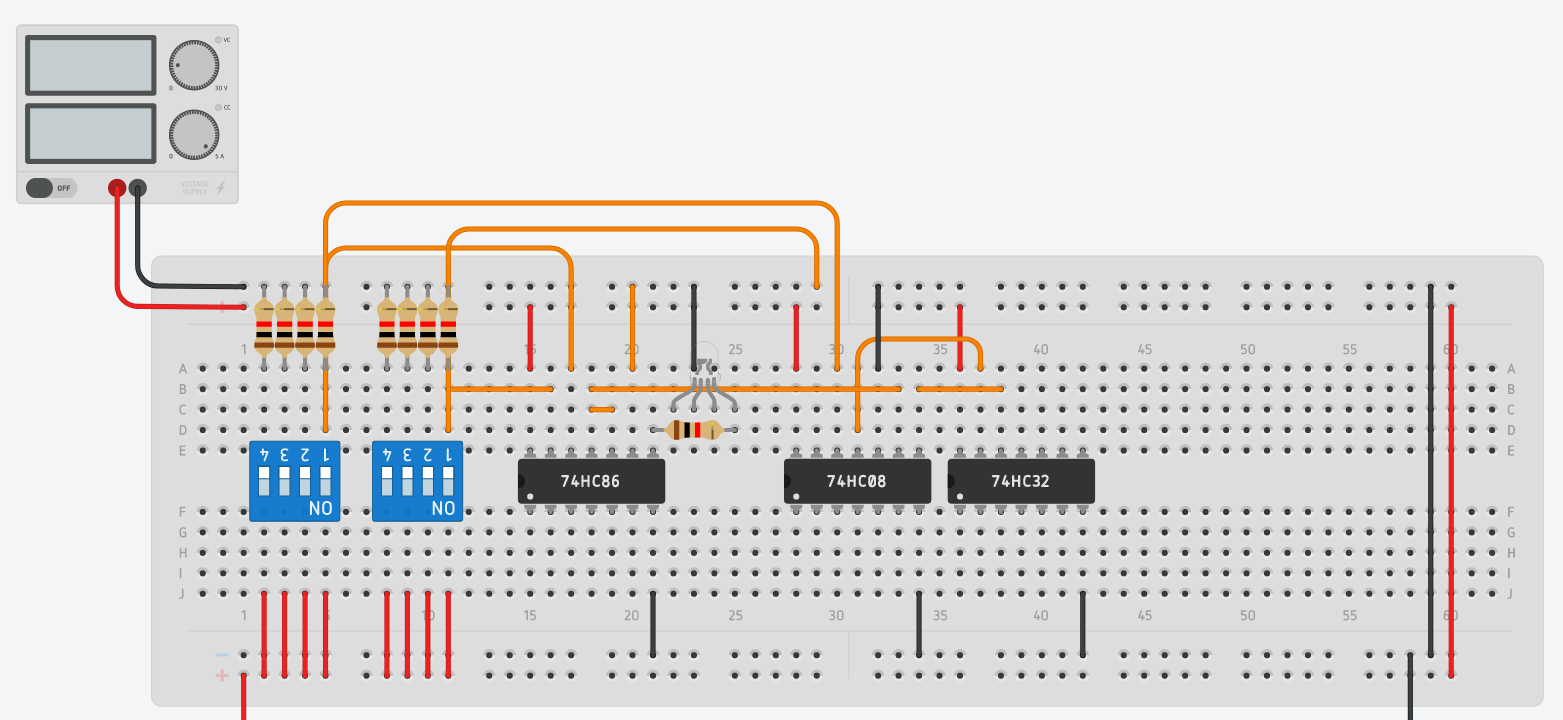
\includegraphics[scale=0.25]{Images/Parte1SC1.png}
	\caption{Primera suma con su correspondiente bit de acarreo.}
	\label{p1sc1}
\end{figure}

\subsubsection{Bitácora 2}

Se realizaron los sumadores de los dos bits restantes y sus correspondientes bits de acarreo. Se tiene un problema con los bits de acarreo y el de desbordamiento, puesto que no encienden todos.

\begin{figure}[H]
	\centering
	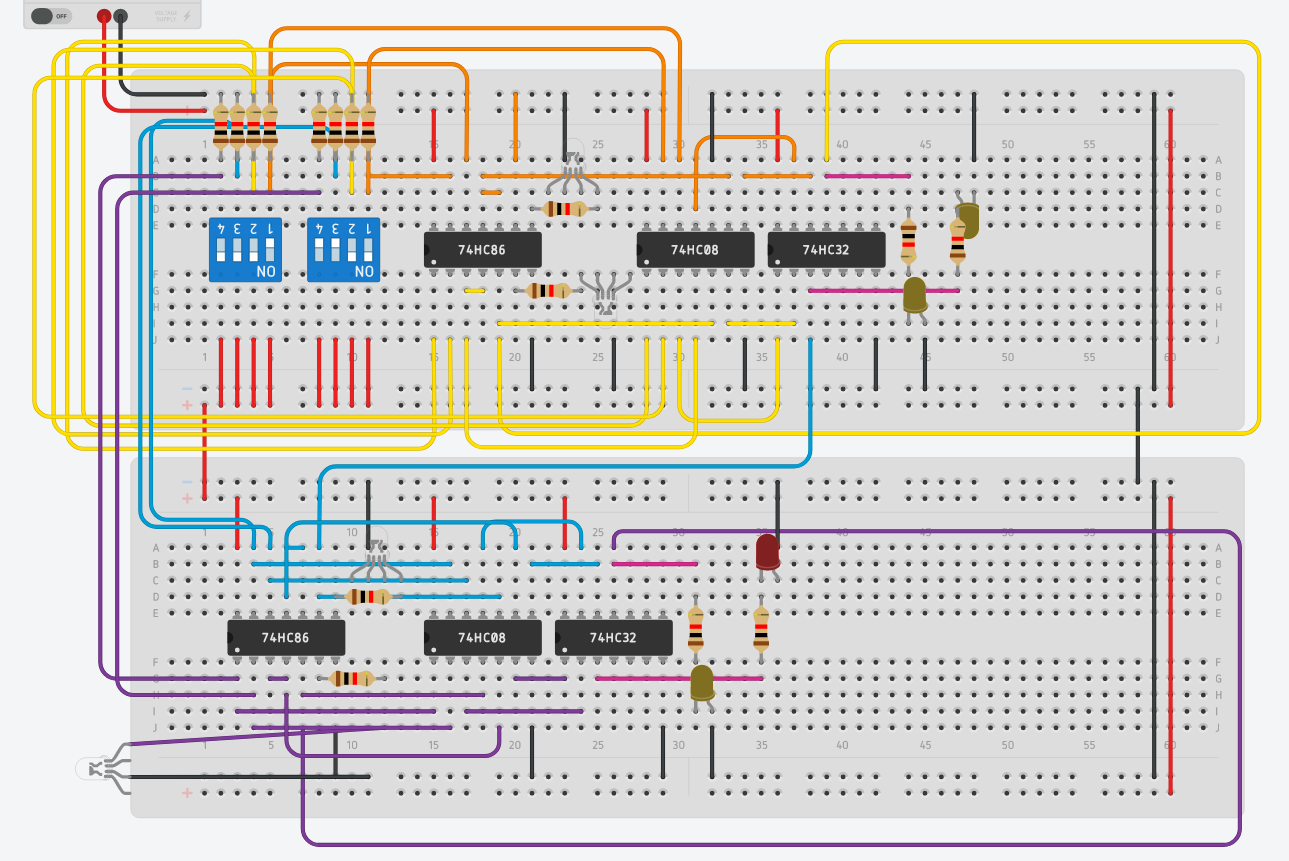
\includegraphics[scale=0.25]{Images/Parte1SC2.png}
	\caption{Circuito Sumador completo para dos sets de $4$ bits con sus bits de acarreo y desbordamiento.}
	\label{p1sc2}
\end{figure}




\subsection{Problema 1}
\subsubsection{Bitácora 3}

Se inició investigando la compuerta 74HC283, el sumador. se implemento la suma de 2 sets de 4 bits. Utilizando dicha compuerta se tiene el siguiente circuito:

\begin{figure}[H]
	\centering
	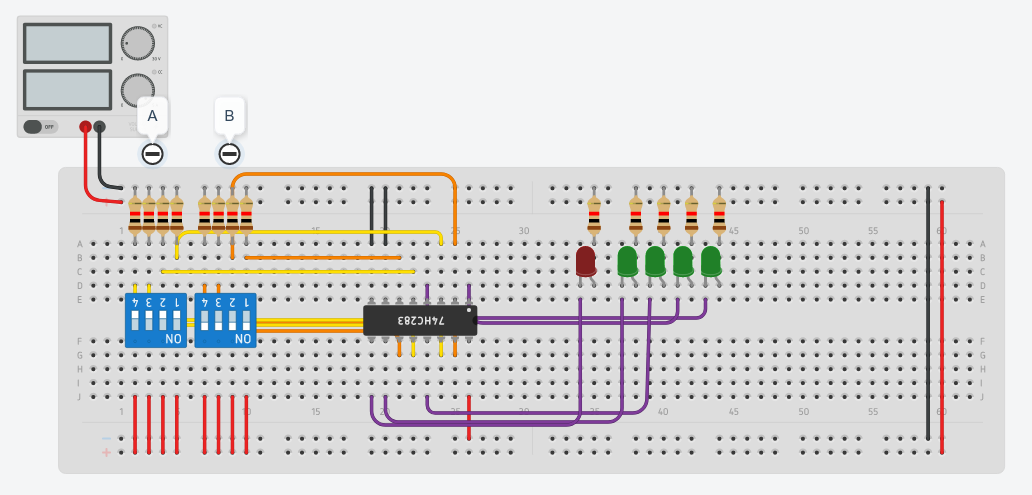
\includegraphics[scale=0.5]{Images/Parte2SC1.png}
	\caption{Circuito sumador con compuerta 74HC283 y los bits de resultado en orden.}
	\label{p2sc1}
\end{figure}


\subsubsection{Bitácora 4}
Por atrasos personales en la práctica no logré realizar la parte de la memoria ni el restador.















